\chapter{Method}

\section{Spent Fuel Conditioning Model}
\subsection{Capabilities}
The spent fuel conditioning model accepts spent fuel bundles and 
packages them into a cylindrical waste packages with user-defined
parameters. 
Each waste package will have a notion of when it was packaged. 

\subsection{Input Variables}
In the spent fuel conditioning model, the user can define the 
variables: 
For each layer, 
\begin{itemize}
	\item thickness
	\item thermal conductivity 
	\item thermal diffusivity
\end{itemize}

For each package,
\begin{itemize}
	\item Number of spent fuel bundles
	\item Radius and height
\end{itemize}

For the facility,  
\begin{itemize}
	\item Throughput 
\end{itemize}

\section{Interim Storage Facility Model}
\subsection{Capabilities}
The interim storage facility accepts waste packages from
spent fuel conditioning facilities. 
It acts as a storage facility and will send waste packages to 
the repository facility based on a loading strategy. 
Various loading strategy logics are included in the interim 
storage facility model. 

\subsection{Loading Strategies}
The loading strategies included in the interim storage facility 
model are: 
\begin{itemize}
\item First Out First In 
\item Last Out First In 
\item Temperature Grouping
\end{itemize}

[** Loading Strategy Literature Review]

\subsection{Input Variables}
In the interim storage facility model, the user can define the 
variables: 
\begin{itemize}
	\item Loading strategy 
	\item Throughput 
	\item Storage time 
\end{itemize} 

\section{Repository Model}

\subsection{Capabilities}
The repository facility emplaces waste canisters in the repository 
in a systematic order: 
\begin{itemize}
    \item emplaces canister in the inner most available space 
    in the available drift until the drift is full 
    \item When drift is full, it starts a new drift
\end{itemize}
It only accepts canisters that results in the temperature limit at
interface between waste package surface and each host geology 
remaining below the thermal limit of the host geologic media. 
Table \ref{tab:temp_limit} shows the temperature limits, thermal 
conductivity and thermal diffusivity for the host geology included 
in the model. 
The repository model will provide the user with a spatial and time 
dependent temperature distribution in the repository. 

\begin{table}[h]
    \centering
	\label{tab:temp_limit}
    \caption{Temperature limit at interface between waste package 
    surface and each host geology \cite{sutton_investigations_2011}}
	\begin{tabular}{|l|l|l|l|}
	\hline
	Rock Type & $T_{limit}$ [$^\circ$C] & k [$\frac{W}{mK}$] &  $\alpha$ [$\frac{m^2}{s}$]  \\ \hline
	Granite   & 100 & 2.5  & $1.13*10^{-6}$\\ \hline
	Clay      & 100 & 1.75 & $6.45*10^{-7}$\\ \hline
	Salt      & 200 & 4.2  & $2.07*10^{-6}$\\ \hline
	\end{tabular}
\end{table}

\subsection{Input Variables}

In the waste repository model, the user can define the variables: 
	\begin{itemize}
		\item Distance between waste packages [m]
		\item Distance between drifts [m]
		\item Repository host geology 
		\item Length of each drift [m]
	\end{itemize}
	
\subsection{Output Tables}
The waste repository model will output the spatial and time 
dependent temperature distribution in the repository in a sqlite 
table. An example of an output table is shown in figure 
\ref{fig:outputtable}. 

\begin{figure}[h]
	\includegraphics[width=0.9\linewidth]{outputtable}
	\caption{Sqlite Table output by \Cyclus showing the spatial and 
	time dependent temperature distribution in the repository}
    \label{fig:outputtable}
\end{figure}

\subsection{Thermal Model}
After the addition of new waste packages at each time step, the 
waste repository model recalculates the temperature at each location
in the repository. 
If the addition of this new package causes its temperature to exceed
the thermal limit, it will be placed back into the buffer. 
A thermal model that relies on a transient `outside' model and 
quasi-steady-state `inside' model is used to accurately determine 
the temperature in the repository \cite{sutton_investigations_2011}.

[** What type of repository design can use this math]

\noindent
\textbf{Transient Outside Model}

The `outside' model assumes a homogenous medium with the \gls{EBS} 
replaced by the geologic medium. 
Figure \ref{fig:conceptual_layout} shows the conceptual layout of 
the central waste package and the adjacent point and line sources. 
The x-axis is along the axial direction, the z-axis is along the 
lateral direction and the y-axis is out of the page. 
For this repository model, a 2D model on the x-z plane is assumed. 

\begin{figure}[h]
	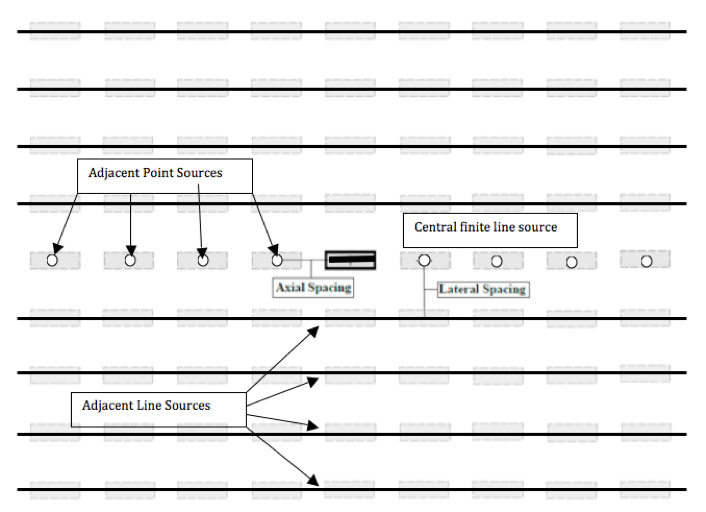
\includegraphics[width=0.9\linewidth]{outsidemodel}
	\caption{Outside Model: Conceptual layout of the central waste 
	package, its adjacent point sources and adjacent line sources 
	\cite{sutton_investigations_2011}}
    \label{fig:conceptual_layout}
\end{figure}

Temperature solutions for the central waste package, adjacent point
and line sources are superimposed to calculate the temperature at 
specific points in the repository.
The equations for calculating temperature of each contributing 
component are included below \cite{sutton_investigations_2011,
greenberg_application_2012,huff_numerical_2012}. 

The central drift consists of one finite line source which 
represents the central waste package. 

\begin{align}
	T_{line}(t,x,y,z) &= \frac{1}{8 \pi k}  \int_{0}^{t} 
	\frac{q_L(t')}{t-t'}e^{\frac{-(x^2+z^2)}{4\alpha(t-t')}} \\
	&[erf[\frac{1}{2}\frac{y+L/2}{\sqrt{\alpha(t-t')}}]-
	erf[\frac{1}{2}\frac{y-L/2}{\sqrt{\alpha(t-t')}}]] dt'
\end{align}

The central drift also consists of point sources that represent 
neighboring waste packages in the central drift. 

\begin{align}
	T_{point}(t,r) = \frac{1}{8 k \sqrt{\alpha} \pi^{3/2}} 
	\int_{0}^{t}\frac{q(t')}{(t-t')^{3/2}}e^{\frac{-r^2}
	{4\alpha(t-t')}}dt'
\end{align}

where $r^2 = (x-x_0)^2 + (y-y_0)^2 + (z-z_0)^2$. 
This can be reduced to $r^2 = (x-x_0)^2$ since the repository in 
this thesis is assumed to be 2D and the point sources in the central 
drift are in the same z-axis.  

The neighboring drifts are represented by infinite line sources.  

\begin{align}
	T_{\infty line}(t,x,z) = \frac{1}{4\pi k} \int_0^t 
	\frac{q_L(t')}{t-t'} e^{\frac{-(x^2+z^2)}{4\alpha (t-t')}} dt'
\end{align}

\subsection{Implementation in \Cyclus}
These equations were implemented in \Cyclus using the boost 
integration libraries to numerically solve the integration.  
